\chapter{Evaluation of the improvements}

To conclude the work, we will evaluate the optimization.  We will study the overhead and the impact of the hybridization of the code and the ideal grainsize. Then we will determine the improvement of the DLB version against the vanilla version.

For all the data showed in this chapter, the timing is the average of the average of 4 time steps of 5 runs. 

\begin{tcolorbox}[colback=yellow!10!white,colframe=red!75!black,title=Important]
  All plots and timing data is presented as a factor from the original. Absolute timing is confidential and we are not allowed to share it.
\end{tcolorbox}

Equation \ref{eq:factor} shows how we compute the timing factor, assume $X$ is the absolute time of the Intel MPI vanilla version and $X'$ is the absolute time for a new version we are presenting. The timing factor ($F_X$) is the quotient between the last and the first. Meaning that if the value is 2, it means it takes the double to compute if the value is 0.5, it takes the half to compute.

\begin{equation}\label{eq:factor}
  F_X=\frac{X'}{X}
\end{equation}

\section{Hybrid version analysis}

Figure \ref{fig:plot-hybrid-int} shows a comparison between the vanilla and the hybrid version on both inputs. We tested different hybrid configurations and grain sizes. First, we can observe both cases that hybridizing does not add overheads. We can compare the \textit{48x1} and the \textit{48x0} configurations and see that the time is nearly equal excepting the reduced case with grain size one that the number of tasks is high and increments the execution time notably. In general terms, hybridization improves the integration time because OmpSs allows improving the load balance among threads. On the detailed case (Figure \ref{fig:plot-hybrid-int-det}) we perceive that the grain size does not impact the performance, although we identify the value 32 as the ideal. The best hybrid configuration for the detailed case is \textit{6x8}. On the reduced case (Figure \ref{fig:plot-hybrid-int-red}) we observe grain size affects the performance. Low grainsize values make the number of tasks increase which adds overhead from making the runtime process tasks. The grainsize values that best fit is greater than 4. The ideal hybrid configuration is \textit{4x12}.

\begin{figure}[ht]
  \begin{subfigure}{1\textwidth}
    \centering
    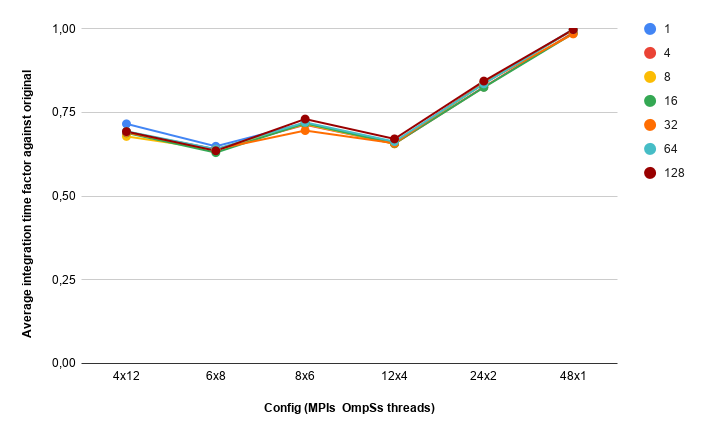
\includegraphics[width=0.7\textwidth]{graphics/hybridcomplete.png}
    \subcaption{Detailed chemistry case}
    \label{fig:plot-hybrid-int-det}

  \end{subfigure}
  \begin{subfigure}{1\textwidth}
    \centering
    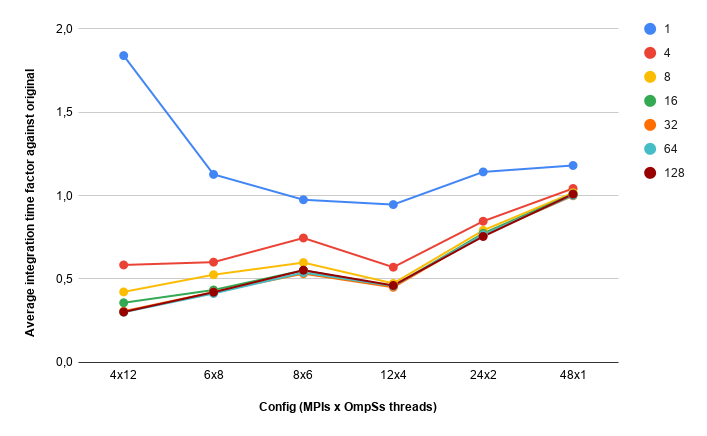
\includegraphics[width=0.7\textwidth]{graphics/hybridreduced.png}
    \subcaption{Reduced chemistry case}
    \label{fig:plot-hybrid-int-red}

  \end{subfigure}

  \caption[Hybrid chemical integration timing comparison.]{Hybrid chemical integration timing comparison. Own compilation.}
  \label{fig:plot-hybrid-int}
\end{figure}

Although hybridization improves the integration time sustainably, the application performance is diminished. 
Figure \ref{fig:plot-hybrid-int-it} shows the same plot but comparing against the iteration time. We can observe that hybridization reduces overall performance. The whole application not being hybridized causes an inefficient usage of the resources and adds unnecessary overheads. This fact makes that we decide to use \textit{48x1} version in both cases as the best for adding DLB. The negative impact of hybridization is higher on the reduced chemistry (Figure \ref{fig:plot-hybrid-int-red-it}) as the integration time weight is lower.

\begin{figure}[ht]
  \begin{subfigure}{1\textwidth}
    \centering
    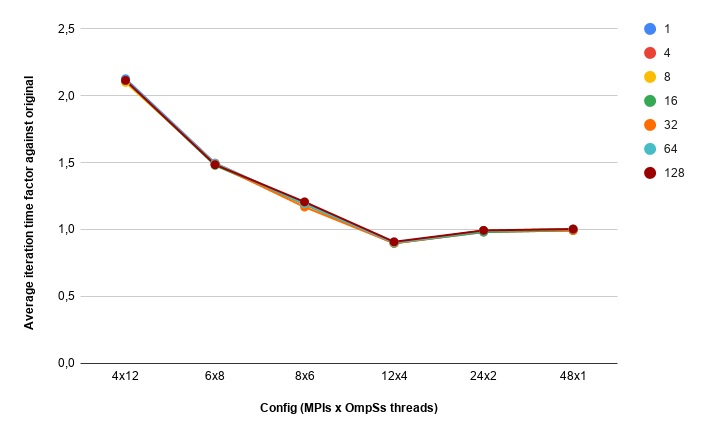
\includegraphics[width=0.7\textwidth]{graphics/hybridcompleteabs.png}
    \subcaption{Detailed chemistry case}

  \end{subfigure}
  \begin{subfigure}{1\textwidth}
    \centering
    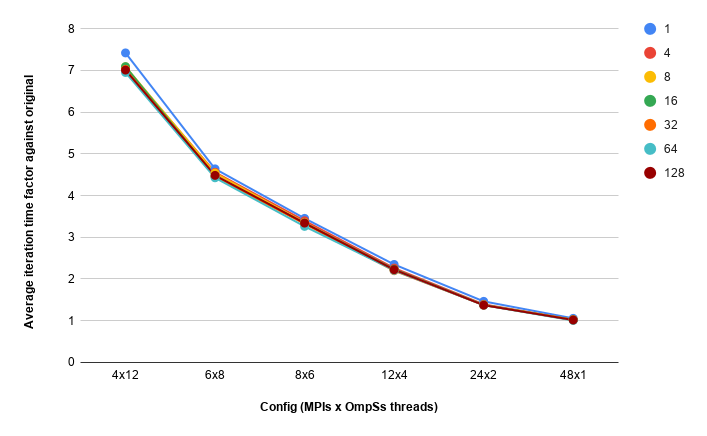
\includegraphics[width=0.7\textwidth]{graphics/hybridreducedabs.png}
    \subcaption{Reduced chemistry case}
    \label{fig:plot-hybrid-int-red-it}

  \end{subfigure}

  \caption[Hybrid iteration timing comparison.]{Hybrid iteration timing comparison. Own compilation.}
  \label{fig:plot-hybrid-int-it}
\end{figure}



\section{DLB version analysis}

In Figure \ref{fig:plot-hybrid-dlb-int}, we compare the integration time between the hybrid version and the DLB version on the configurations we tested in the previous section. This time, we don't check all grainsize values. Instead, we choose the ideal for each input. We can observe that applying DLB makes all configurations faster than the pure MPI version and all the hybrid configurations. It is also remarkable that there is no notable difference between hybrid configurations. On the detailed chemistry (Figure \ref{fig:plot-hybrid-dlb-int-det}) we see that with DLB we achieve a \textit{x2} respect the original. On the reduced chemistry (Figure \ref{fig:plot-hybrid-dlb-int-red}) we achieve a \textit{x7} with DLB on the best configuration (\textit{12x4}). Nonetheless, with the \textit{48x1} configuration, we achieve a \textit{x5} speedup against original.
\begin{figure}[ht]
  \begin{subfigure}{1\textwidth}
    \centering
    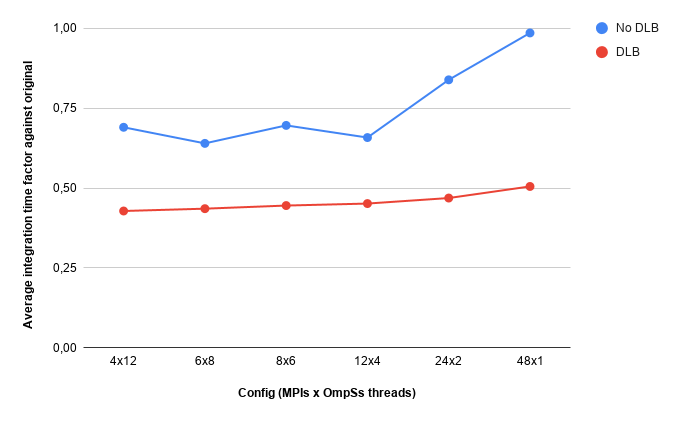
\includegraphics[width=0.7\textwidth]{graphics/hybridcompletedlb.png}
    \subcaption{Detailed chemistry case}
    \label{fig:plot-hybrid-dlb-int-det}

  \end{subfigure}
  \begin{subfigure}{1\textwidth}
    \centering
    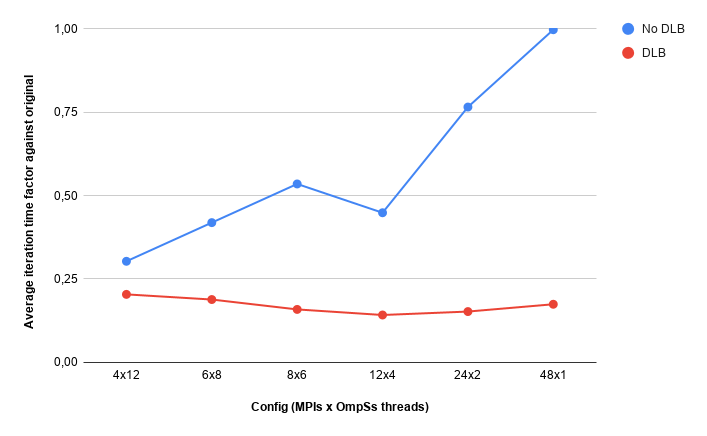
\includegraphics[width=0.7\textwidth]{graphics/hybridreduceddlb.png}
    \subcaption{Reduced chemistry case}
    \label{fig:plot-hybrid-dlb-int-red}

  \end{subfigure}

  \caption[DLB chemical integration time factor on hybrid configurations.]{DLB chemical integration time factor on hybrid configurations. Own compilation.}
  \label{fig:plot-hybrid-dlb-int}
\end{figure}

To see the overall performance, in Figure \ref{fig:plot-hybrid-dlb-it} we compare the average time step with and without DLB on the hybrid configurations with the ideal grainsize. As seen in the previous section, the hybrid configurations are far from the pure MPI version since the application is not fully parallelized with OmpSs. Although, in general terms with the \textit{48x1} configuration, we achieve a speedup in both inputs. On the detailed chemistry case (Figure \ref{fig:plot-hybrid-dlb-it-det}), we earn a \textit{1.5x} speedup. On the reduced chemistry case (Figure \ref{fig:plot-hybrid-dlb-it-red}), as the integration weight is lower, the speedup achieved is \textit{1.3x}.

\begin{figure}[ht]
  \begin{subfigure}{1\textwidth}
    \centering
    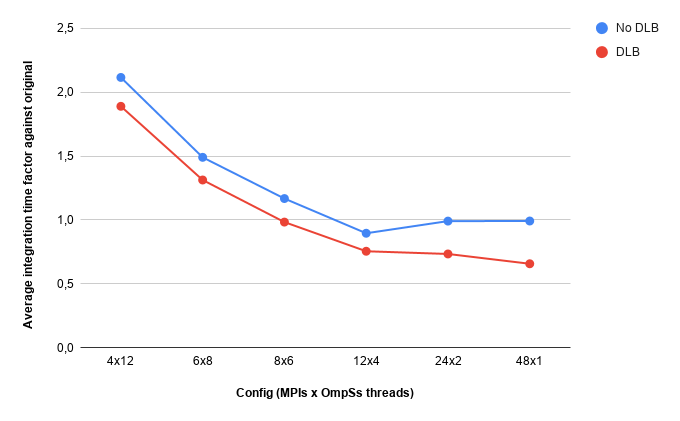
\includegraphics[width=0.7\textwidth]{graphics/hybridcompletedlbabs.png}
    \subcaption{Detailed chemistry case}
    \label{fig:plot-hybrid-dlb-it-det}

  \end{subfigure}
  \begin{subfigure}{1\textwidth}
    \centering
    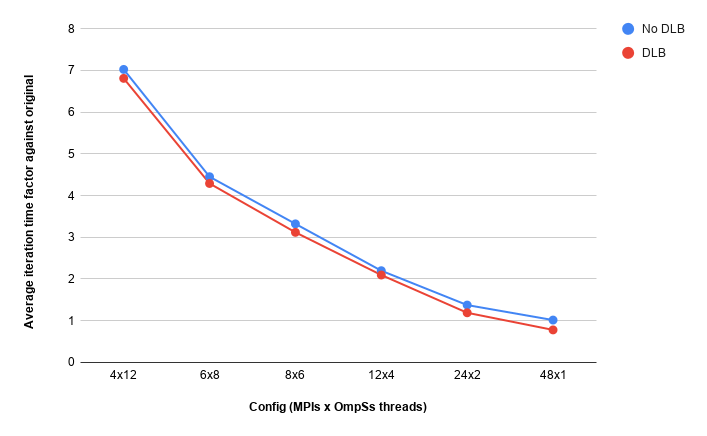
\includegraphics[width=0.7\textwidth]{graphics/hybridreduceddlbabs.png}
    \subcaption{Reduced chemistry case}
    \label{fig:plot-hybrid-dlb-it-red}

  \end{subfigure}

  \caption[DLB iteraiton time factor on hybrid configurations.]{DLB iteration time factor on hybrid configurations. Own compilation.}
  \label{fig:plot-hybrid-dlb-it}
\end{figure}

Now we will check how the optimization behaves when running with multiple nodes. Figure \ref{fig:plot-hybrid-dlb-int-mul} shows the integration time factor running with DLB against the pure MPI version with the same number of processes, both inputs, grainsize 16 for the complete integration and grainsize 32 for the reduced. We can see that in the complete integration case (Figure \ref{fig:plot-hybrid-dlb-int-mul-det}), the speedup is constant to \textit{2x}. On the reduced (Figure \ref{fig:plot-hybrid-dlb-int-mul-red}), DLB effectiveness is lost when increasing the number of nodes. This loss is probably because when we increase the number of nodes, the balance among nodes is worse. DLB can balance the workload difference within a node because it relays on a shared memory programming model. % In the next section, we will identify the problem using a DLB module and handle the issue.

\begin{figure}[ht]
  \begin{subfigure}{1\textwidth}
    \centering
    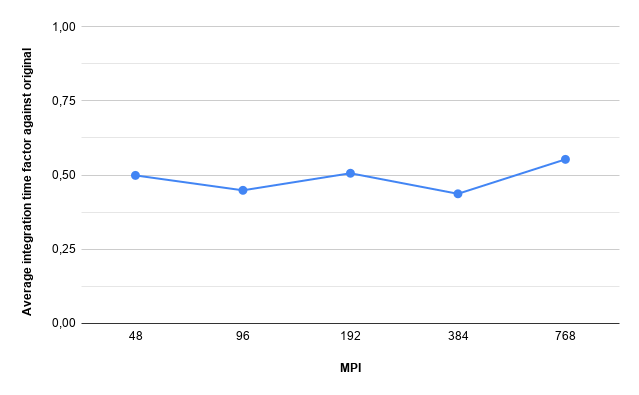
\includegraphics[width=0.7\textwidth]{graphics/hybridcompletedlbmulti.png}
    \subcaption{Detailed chemistry case}
    \label{fig:plot-hybrid-dlb-int-mul-det}

  \end{subfigure}
\begin{subfigure}{1\textwidth}
    \centering
    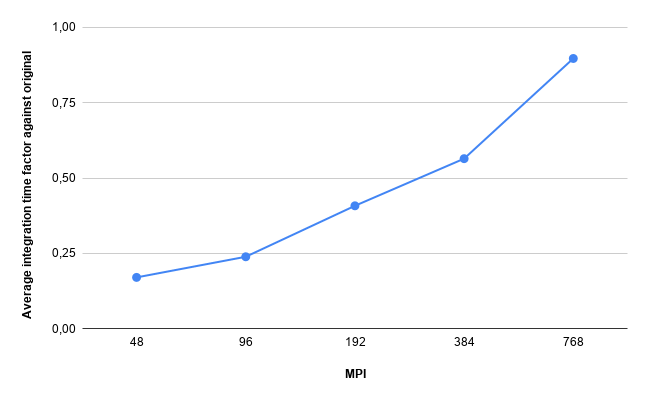
\includegraphics[width=0.7\textwidth]{graphics/hybridreduceddlbmulti.png}
    \subcaption{Reduced chemistry case}
    \label{fig:plot-hybrid-dlb-int-mul-red}

  \end{subfigure}

  \caption[DLB Chemical Integration time factor multinode.]{DLB Chemical Integration time factor multinode. Own compilation.}
  \label{fig:plot-hybrid-dlb-int-mul}
\end{figure}

Figure \ref{fig:plot-hybrid-dlb-int-mul-scal} presents the scalability plots of the same runs, with and without DLB. On the detailed case (Figure \ref{fig:plot-hybrid-dlb-int-mul-scal-det}), we see scalability from both versions are similar. This fact makes sense since the speedup showed in the last plot is constant, the scalability between the versions is analogous. On the reduced chemistry (Figure \ref{fig:plot-hybrid-dlb-int-mul-scal-red}) we observe that the DLB version's scalability is poor because as said, DLB loses effectiveness when increasing the number of processes.

\begin{figure}[ht]
  \begin{subfigure}{1\textwidth}
    \centering
    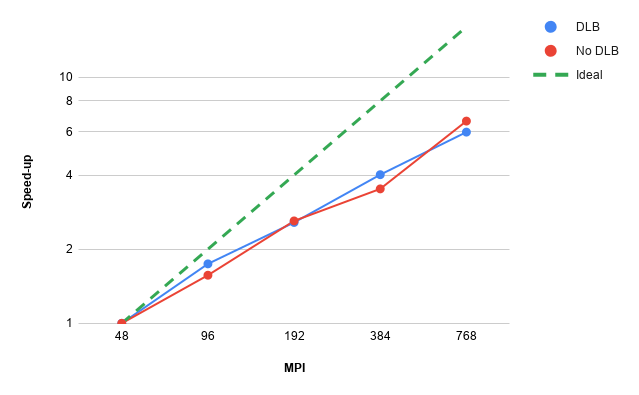
\includegraphics[width=0.7\textwidth]{graphics/hybridcompletedlbmultiscal.png}
    \subcaption{Detailed chemistry case}
    \label{fig:plot-hybrid-dlb-int-mul-scal-det}

  \end{subfigure}
  \begin{subfigure}{1\textwidth}
    \centering
    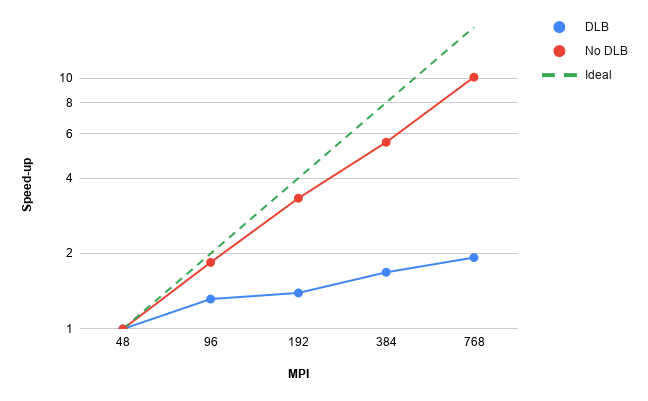
\includegraphics[width=0.7\textwidth]{graphics/hybridreduceddlbmultiscal.png}
    \subcaption{Reduced chemistry case}
    \label{fig:plot-hybrid-dlb-int-mul-scal-red}

  \end{subfigure}

  \caption[Chemical integration scalability comparison]{Chemical integration scalability comparison. Own compilation.}
  \label{fig:plot-hybrid-dlb-int-mul-scal}
\end{figure}

%\section{Tracking Application Life Performance: TALP}




